\documentclass[10pt,twocolumn,letterpaper]{article}

% My own stuff
\usepackage{booktabs}
% \usepackage{caption}
% \captionsetup[table]{skip=8pt}   % Only affects tables
\usepackage{stfloats}  % Add this to the preamble
\usepackage{float}
% \usepackage{cm-super}
\usepackage[T2A]{fontenc}    % Enables Cyrillic fonts
\usepackage[utf8]{inputenc}   % Assumes your source file is in UTF-8 encoding
\usepackage[russian]{babel}   % Loads Russian language support


\usepackage{cvpr}
\usepackage{times}
\usepackage{epsfig}
\usepackage{graphicx}
\usepackage{amsmath}
\usepackage{amssymb}

\makeatletter
\def\cvprsubsection{\@startsection {subsection}{2}{\z@}
    {8pt plus 2pt minus 2pt}{6pt}{\bfseries\normalsize}}
\makeatother

% Include other packages here, before hyperref.

% If you comment hyperref and then uncomment it, you should delete
% egpaper.aux before re-running latex.  (Or just hit 'q' on the first latex
% run, let it finish, and you should be clear).
\usepackage[breaklinks=true,bookmarks=false]{hyperref}

\cvprfinalcopy % *** Uncomment this line for the final submission

\def\cvprPaperID{****} % *** Enter the CVPR Paper ID here
\def\httilde{\mbox{\tt\raisebox{-.5ex}{\symbol{126}}}}

% Pages are numbered in submission mode, and unnumbered in camera-ready
%\ifcvprfinal\pagestyle{empty}\fi
\setcounter{page}{1}
\begin{document}

%%%%%%%%% TITLE
\title{Обоснованный данными ввод в теорию ЕКОД Часть 1/2: Современное понимание теории Джанибекова Колебания Рассоединения «Переворот Земли» Экзотермической Ядро-Мантии (ЕКОД)}

\author{Чжунхо\\
Вебсайт: \href{https://sovrynn.github.io}{sovrynn.github.io}\\
Исследовательский репозиторий ЕКОД: \href{https://github.com/sovrynn/ecdo}{github.com/sovrynn/ecdo}\\
{\tt\small junhobtc@proton.me}
}

\maketitle
%\thispagestyle{empty}

%%%%%%%%% ABSTRACT
\begin{abstract}
В мае 2024 года анонимный онлайн-автор под именем «The Ethical Skeptic» \cite{0} предложил революционную теорию, называемую Экзотермическое Рассоединение Ядро-Мантии Джанибекова Колебания (ЕКОД) \cite{1}. Эта теория предполагает, что Земля ранее испытывала внезапные катастрофические смещения своей оси вращения, вызывая массовые мировые наводнения из-за того, что океаны перераспределялись через континенты вследствие инерции вращения. Кроме того, теория предлагает объяснительный геофизический процесс и данные, указывающие на то, что такой переворот может быть неизбежен. В то время как такие катастрофические наводнения и предсказания конца света не являются новыми, теория ЕКОД уникально убедительна благодаря научному, современному, многодисциплинарному и основанному на данных подходу.

Эта статья является первой частью из двух частей конденсированного резюме полугодичного независимого исследования \cite{2,20} теории ЕКОД. Она подчеркивает три основных момента:

\begin{flushleft}
\begin{enumerate}
    \item Переворот типа ЕКОД уже произошел несколько раз в недавней истории человечества, о чем свидетельствуют мифы о наводнениях и геологические признаки широкомасштабных континентальных наводнений.
    \item Приблизительное направление и величина прошлых переворотов Земли могут быть наглядно определены.
    \item Недавние геомагнитные и геофизические данные предполагают, что еще один переворот Земли может быть неизбежен и что изменения климата могут быть вызваны изменениями глубоко внутри Земли, а не деятельностью человека.
\end{enumerate}
\end{flushleft}

Кроме того, я рассматриваю причинные физические процессы позади предложенного теорией ЕКОД «переворота Земли».

В этой статье я сохраняю объективность, сосредотачиваясь на твердых данных, избегаю убедительных, но гипотетических частей теории и подчеркиваю, что это тема, к которой человечество имеет насущную потребность в дальнейшем исследовании.
\end{abstract}

%%%%%%%%% BODY TEXT
\section{Введение}
\begin{figure}[b]
\begin{center}
   \includegraphics[width=1\linewidth]{b.png}
\end{center}
   \caption{Местоположение историй о потопах по всему миру \cite{3}.}
\label{fig:1}
\label{fig:onecol}
\end{figure}
Истории о великом потопе не новы - на самом деле, они находятся в каждой крупной культуре по всему миру, охватывая все колыбели цивилизации. Построение графика (Рисунок \ref{fig:1}) из 267 историй о потопах \cite{3} показывает, что практически все обитаемые регионы Земли содержат истории о потопах.


Более пристальный взгляд на эти истории о потопах показывает нам, что это были не обычные потопы, а разрушительные катаклизмы, сопровождаемые потопами, которые очищали континенты.

\subsection{Истории Катаклизмов Коренных Американцев}

Истории коренных американцев содержат одни из самых ярких описаний великих катаклизмов Земли. Хопи, племя коренных американцев, которое живет на северо-востоке Аризоны, говорят, что, \textit{"..Сотукнанг призвал Муравьиных Людей открыть их подземный мир для избранных людей. Когда они были в безопасности под землёй, Сотукнанг приказал близнецам, Пёкангхоя и Палоңавхоя, покинуть свои посты на северном и южном концах оси мира, где они находились для поддержания правильного вращения земли. \textbf{Близнецы едва покинули свои посты, как мир, оставшись без контроля, потерял баланс, закрутился безумно, а затем перевернулся дважды.} Горы обрушились в моря с большим всплеском, моря и озера захлестнули сушу, и когда мир закрутился через холодное и безжизненное пространство, замерз в твёрдый лёд"} \cite{4}.

Многие из этих историй точно описывают масштабные наводнения, рассказывая о том, как океаны поднялись, чтобы затопить всё, кроме самых высоких горных вершин. Индеец Скомомиш, живущий в штате Вашингтон, рассказывает, как, \textit{"Великий Дух, разгневанный злобой людей и животных, решил избавиться от земли всех, кроме хороших животных, одного хорошего человека и его семьи. По указанию Великого Духа человек выстрелил стрелой в облако, затем другой стрелой в ту стрелу и так далее, создавая верёвку из стрел от облака до земли. Хорошие животные и люди поднялись наверх. Плохие животные и змеи начали подниматься, но человек оборвал верёвку. \textbf{Затем Великий Дух вызвал много дней дождя, затопивших до снежной линии Тахома (гора Рейнир).} После того как все плохие люди и животные утонули, Великий Дух остановил дождь, вода медленно спала, и хорошие люди и животные спустились вниз"} \cite{3}. Для справки, гора Рейнир - это активный вулкан в Вашингтоне с высотой вершины 4392,5 м над уровнем моря.

История о наводнении у индейцев Маках из штата Вашингтон конкретно упоминает многофазное наводнение из "очень тёплых" вод, указывая на то, что это не было обычным наводнением: \textit{"Океан поднялся настолько высоко, что отрезал мыс. Затем он отступил, достигнув низкого уровня через четыре дня, оставив бухту Ниа сухой. Затем он снова поднялся, чтобы покрыть всё, кроме горных вершин. \textbf{Поднимающиеся воды были очень теплыми.} Люди с каноэ загрузили свою собственность и были унесены далеко на север. Многие погибли, когда их каноэ запутались в деревьях. Море вернулось к норме ещё через четыре дня, и люди обнаружили себя далеко на севере, где их потомки всё ещё живут"} \cite{3}.

\subsection{Китайские истории катаклизмов}

На противоположной стороне Тихого океана считается, что современная китайская цивилизация началась с великого потопа. Династия Ся, предположительно существовавшая около 2000 года до нашей эры, была создана Великим Юем, который остановил Великий Потоп Гун-Юй \cite{6}. В его время, \textit{"...говорят, произошло чудо, что солнце на протяжении десяти дней не заходило, леса были подожжены, и появилось множество отвратительных вредителей... Огромная волна, "достигшая неба", обрушилась на землю Китая. \textbf{"Воды поднимались высоко на горы, и предгорья были совершенно не видны"}... "Разрушительным в своем разливе являются воды наводнения", - сказал император. "В своем обширном размахе они охватывают холмы и накрывают великие высоты, угрожая небесам своими потоками". Император приказал приложить все усилия, чтобы открыть выходы для вод, застрявших в долинах между горами. На протяжении многих лет население работало, пытаясь освободить равнины и долины от вод потопа, выкапывая каналы и осушая поля. На протяжении значительного числа лет все усилия были напрасны. Министр, ответственный за эту срочную и огромную работу, Хуан, был приговорен к смерти из-за его провала... и только его сын Юй преуспел в осушении земли. Этот подвиг был настолько высоко оценен, что Юй стал императором Китая после короля Шуня, первого преемника Яхоу"} \cite{5}.

Казалось бы, не только Китай был затоплен, но и возникла необходимость перемерить стороны света и движения солнца и луны, что подразумевает, что вращение Земли могло измениться во время наводнения: \textit{\textbf{"Этот император отправил ученых в разные части Китая и даже в Индокитай, чтобы выяснить расположение севера, запада, востока и юга, наблюдая направление восхода и захода солнца и движение звезд.} Он также поручил своим астрономам выяснить длительность сезонов и составить новый календарь... "После этого Яоу [Яхоу] приказал Хэ и Хо в благоговении согласно широким небесам, вычислить и очертить движения и появления солнца, луны, звезд и зодиакальных пространств; и уважительно передать сезоны народу""} \cite{5}.

Записи о катаклизмах в китайской истории на самом деле восходят задолго до династии Ся, достигая периода Трех Суверенов и Пяти Императоров \cite{7}. Нюйва, один из Трех Суверенов и центральная фигура сотворения в китайской истории, остановила потоп во время катаклизма, когда Земля изменила свое вращение: \textit{"Произошла ссора между двумя более могущественными богами, и они решили выяснить её в бою. Когда бог воды Гун Гун увидел, что проигрывает, он разбил свою голову о гору Бучжоу, столб, поддерживающий небо. \textbf{Столб рухнул, и это вызвало наклон неба к северо-западу и смещение земли к юго-востоку.} Это вызвало великие бедствия, такие как нескончаемые пожары, обширные наводнения и появление свирепых людоедов. Нюйва отрезала ноги гигантской черепахи и использовала их, чтобы заменить упавший столб, облегчая ситуацию и запечатывая разрушенное небо камнями семи различных цветов, но она не смогла полностью исправить наклоненное небо"} \cite{8}.

\subsection{Европейские, майя, ближневосточные и юго-восточные азиатские истории о катаклизмах}

Поскольку историй катастроф слишком много, чтобы подробно описывать их в этой работе, я упомяну кратко о некоторых других известных культурах с такими историями. Греческая литература содержит три истории о потопах: Девкалиона, Огигеса и Дардана \cite{9,10}. Во время первого из них, \textit{"Через девять дней потопа, мир был разрушен, и ковчег остановился на вершине горы Парнас"}, высота которой составляет 2 457 метров \cite{11}. В литературе майя считается, что перед текущим Солнцем было четыре разных Солнца, и что век четвертого Солнца, Кальчиутликуэ, закончился всемирным потопом около 3100 года до н.э. и рождением текущего пятого солнца \cite{12}. На Ближнем Востоке библейская хронология содержит знаменитый потоп Ноя, а "Эпос о Гильгамеше", вавилонская поэма, рассказывает аналогичную историю \cite{13}. Культуры Юго-Восточной Азии также богаты историями о потопах - например, народ От Данум из Индонезии говорит, что, \textit{"Великий потоп однажды утопил много людей. Немногие уцелели, спасшись на лодках на единственную оставшуюся над водой вершину горы. Они проживали там три месяца, пока потоп не спал"} \cite{3}. Остров Борнео, на котором они живут, имеет максимальную высоту 4 095 метров.

\begin{figure*}[t]
\begin{center}
% \fbox{\rule{0pt}{2in} \rule{.9\linewidth}{0pt}}
\includegraphics[width=1\textwidth]{marine.jpg}
\end{center}
   \caption{Глобальное распределение морских (океанических) окаменелостей, солей и соляных равнин/шахт \cite{15,16,86,87}.}
   \label{fig:2}
\end{figure*}

\subsection{Статистический анализ историй о катастрофах}

Очевидно, эти истории описывают потопы, которые зачастую сопровождались другими видами катастрофических геофизических сил. Анализ 117 историй о катастрофах (Таблица \ref{tab: 1}) показывает, что огненные бури, топографические изменения и изменения в вращении Земли часто упоминаются как события, происходившие вместе с великими наводнениями \cite{14}:

\begin{table}[ht]
\begin{center}
\renewcommand{\arraystretch}{1.2}  % Optional, to increase row spacing
\begin{tabular}{|l|c|c|}
\hline
\textbf{Тип катастрофы} & \textbf{Количество} & \textbf{\%} \\
\hline\hline
Потоп/наводнение        & 84 & 71.79 \\
Пожар/огненная буря     & 39 & 33.33 \\
Ландшафтные сдвиги & 29 & 24.79 \\
Звездное расстройство   & 15 & 12.82 \\
Обрушившееся небо       & 15 & 12.82 \\
Продолжительная темнота & 14 & 11.97 \\
Потерянные земли и озера & 12 & 10.26 \\
Циклонные ветры         & 10 & 8.55  \\
Осевая перемена & 9 & 7.69  \\
Кипящие реки/океаны & 8 & 6.84 \\
\hline
\end{tabular}
\end{center}
\caption{Частота катастрофических эффектов в историях}
\label{tab: 1}
\end{table}

Конкретность историй о потопах, возникающих из множества независимых культур по всему миру, вместе с совпадающими историями о других катастрофических событиях, предполагают, что эти истории о потопах могут быть прямыми свидетельствами реально произошедших катастроф.

\section{Физические доказательства океанического потопа}

Подтверждают истории о потопах различные виды физических доказательств широкомасштабного океанического затопления, лежащие на поверхности континентальных масс Земли. Самыми прямыми из таких видов доказательств являются соли (морская вода, соляные равнины и шахты) и морские (океанические) окаменелости, которые покрывают большие площади континентальных земель Земли. Рисунок \ref

Некоторые из самых интересных областей, содержащих соленую воду, находятся в Гималайских возвышенностях Тибета и в Андах Южной Америки, обе области на средней высоте 4000 метров, причем первая изображена на Рисунке \ref{fig:3}. Легенды о наводнениях в Тибете говорят, что, \textit{"\textbf{Тибет был почти полностью затоплен}, пока бог Гьян не зажалился над выжившими, не отводя воды через Бенгалию, и не послал учителей, чтобы цивилизовать людей, которые до тех пор были мало чем лучше обезьян"} \cite{3}. Перуанские мифы описывают строительство гор, происходящее одновременно с наводнениями на вершинах гор: \textit{"Пастух и его шестеро детей собрали всю еду и овец, которые могли, и взяли их на вершину очень высокой горы Анкасмарка. \textbf{Когда вода поднималась, гора поднималась выше, так что ее вершина никогда не была затоплена, а позже гора опустилась вместе с водой.} Шестеро детей заселили провинцию после наводнения"} \cite{3}.

\begin{figure}[t]
\begin{center}
   \includegraphics[width=1\linewidth]{tibet.jpg}
\end{center}
   \caption{Топографическая карта Гималаев, изображающая соленую воду (бирюзовый), высохшую соль (белый) и морские окаменелости (красный) \cite{15,16,86,87}.}
\label{fig:3}
\label{fig:onecol}
\end{figure}

Пока униформитарная школа геологической мысли приписывает аномалии, такие как соль и морские окаменелости, длительным процессам, происходящим на протяжении миллионов лет, истории о наводнениях человечества должны заставить нас усомниться в этом направлении мышления. Если океан на самом деле заливает континенты, то соленая вода и морские окаменелости, легко обнаруживаемые на обширных массивах высокогорных земель, именно то, что мы и ожидали найти.

\begin{figure*}[b]
\begin{center}
\includegraphics[width=0.85\textwidth]{khafre.jpg}
\end{center}
   \caption{Диаграмма, показывающая дифференциальную, узорчатую эрозию карста, вызванную устойчивым временным подъемом уровня моря \cite{27}.}
\label{fig:4}
\end{figure*}

\subsection{Дополнительные физические аномалии}

Существует множество других форм аномалий, которые униформитарная наука не может объяснить. Идеально сохранившиеся, мгновенно замороженные мамонты, захороненные в грязи с мясом, все еще пригодным для употребления через тысячи лет \cite{17,18,19}, огромные пласты горизонтально уложенного осадка в Северной Америке, охватывающие 2,4 млн км$^2$ \cite{21}, ландшафты с волнами мега-течений \cite{22}, и валуны, происходящие из сотен километров и лежащие на вершинах гор \cite{23,26} - всего лишь часть явлений, которые современная униформитарная геология просто отмахивается, используя всеобъясняющие объяснения "длительных, растянутых процессов". Таких аномалий лучше всего объяснить через катастрофические геофизические силы, и они исследованы во второй части этой статьи.

Дополнительно, отклонения и реверсы геомагнитных полюсов широко признаны, как повторяющееся явление Земли, основанное на палеомагнитных данных \cite{35,40,41}. Однако современная наука не объясняет, почему и как происходят эти реверсы полюсов.

\section{ЭЦДО и пирамиды Гизы}

Пирамиды Хафры и Хуфу в Гизе являются одной из ключевых фокусных точек в тезисе Этического скептика по ЭЦДО \cite{27}, поскольку они не только предоставляют доказательства устойчивого временного затопления океаном, но и указывают на потенциальное направление перемен ЭЦДО Земли, предполагая, что наши предки могли измерять катаклизмы Земли и обладали инженерными навыками, чтобы зафиксировать это знание в массивных, высокоточно спроектированных каменных структурах. Эти две пирамиды, предположительно построенные около 2500 г. до н.э. в качестве гробниц для фараонов Хуфу и Хафры, обе расположены на севере Египта в точке приблизительно (30 N, 31 E). Их основания более чем 200 метров в длину, а высота около 140 метров. Пирамида Хуфу была построена с использованием около 2,3 миллионов известняковых блоков, каждый из которых весил в среднем более двух тонн \cite{24, 25}.

Существует значительная неопределенность в отношении происхождения этих пирамид, которую Ethical Skeptic освещает в своей диссертации. Он указывает на многочисленные несоответствия в традиционном повествовании о пирамидах, указывая, в лучшем случае, на значительную путаницу в отношении возраста и истории пирамид:

\begin{flushleft}
\begin{itemize}
    \item Радиоуглеродное датирование древних растворов и инструментов грабителей гробниц поблизости указывает на то, что пирамиды, вероятно, были построены гораздо раньше, чем это принято считать.
    \item Так называемые "каменоломенные отметки", найденные в внутренних камерах пирамиды Хеопса, вызывают подозрения из-за их расположения, материала, состояния сохранности, использования египетских иероглифов и времени/характера обнаружения, что указывает на то, что это могут быть подделки. Они также отличаются от других подлинных древних охристых отметок, найденных в другой части пирамиды.
    \item Дифференциальная карстовая эрозия на близлежащем Сфинксе не согласуется с общепринятой версией его строительства.
\end{itemize}
\end{flushleft}

\begin{figure*}[b]
\begin{center}
\includegraphics[width=0.85\textwidth]{shafts.jpg}
\end{center}
   \caption{Внутренние шахты и камеры пирамиды Хеопса, которые, как предполагает Ethical Skeptic, представляли собой трёхчастную геофизическую обсерваторию для мониторинга событий ECDO \cite{28}.}
\label{fig:5}
\end{figure*}

Одной из ключевых областей исследования в диссертации Ethical Skeptic является дифференциальная, узорчатая эрозия на внешней стороне пирамиды Хефрена, изображённой на рисунке \ref{fig:4}. Верхушка пирамиды сохраняет свою первоначальную мягкую облицовку из известняка Тура, которая когда-то покрывала всю пирамиду. Эта облицовка из известняка слегка выветрена, но расположена прямо над узким, сильно карстовым эрозионным слоем, обнажающим более твёрдый известняк Моккатам с твёрдостью 7 по Моосу, использовавшийся для внутренних структурных блоков пирамиды. Ниже этого тела пирамиды сохраняется сильно карстовый эрозионный слой из известняка Тура с твёрдостью 4 по Моосу. Ключевой момент здесь заключается в том, что более мягкий известняк Тура, использовавшийся для внешней облицовки пирамиды, содержащий CaCO$_3$, может растворяться в воде при определённых условиях. Ethical Skeptic ссылается на избирательное сильное карстовое размывание, останавливающееся на твёрдом известняке Моккатам, волнообразную эрозию на углах вершины и различие между лёгким выветриванием возвышенной вершины и сильной карстовой эрозией нижней части пирамиды, как на явные доказательства продолжительного подъёма уровня океана, который также быстро отступил \cite{27}.

\begin{figure*}[b]
\begin{center}
\includegraphics[width=1\textwidth]{drawing.jpg}
\end{center}
   \caption{Изображение предполагаемого вращения ECDO, идущего на 104 градуса к северу вдоль 31-го восточного меридиана, с крестами, обозначающими восточные и западные поворотные точки, и красным маркером, обозначающим пирамиду Хеопса.}
\label{fig:6}
\end{figure*}

Ethical Skeptic также уделяет значительное внимание внутреннему дизайну и состоянию пирамиды Хеопса (рисунок \ref{fig:5}) в своём исследовании \cite{28}. Пирамида Хеопса содержит несколько камер (Царская, Царицы и Подземная камеры), различные коридоры и шахты, а также две пары так называемых "воздушных шахт", по одной паре, выходящей из каждой из Царской и Царицыной камер \cite{29,30}. В этой работе мы рассмотрим только самые важные части исследования Ethical Skeptic - ориентацию и дизайн двух пар "воздушных шахт", так как они содержат важную информацию о направлении переворотов ECDO Земли.

Ключевой момент здесь заключается в понимании того, что шахты были построены с очень точной ориентацией на определённые направления. Во-первых, обе пары шахт в настоящее время устремлены точно на север и юг. Кроме того, они были построены с внутренним углом 104 градуса.

Наиболее убедительная улика, однако, это небесная звездная карта, вырезанная на внутренней стороне одного из королевских шахт. Эта звездная карта сосредоточена вокруг небесной ориентации северного полюса с приблизительно 9600 по 9200 годы до нашей эры, основываясь на прецессии равноденствий \cite{28}. Это предполагает преднамеренную ориентацию шахт, и что во время строительства одна пара шахт из Камеры Короля и Королевы указывала на небесный северный полюс. Это ставит вопрос - на что указывают другие концы шахт, и почему они оба были построены с углом в 104 градуса? Ethical Skeptic предполагает, что они были построены для того, чтобы сориентироваться на небесный северный полюс после 104-градусного поворота ECDO.

\section{Доказательства 104-градусного вращения вдоль 31-го меридиана}

Таким образом, Ethical Skeptic предполагает, что Земля испытывает периодические 104-градусные перевороты вдоль 31-го меридиана, вдоль которого расположена пирамида Хеопса и ее двойные шахты. Рисунок \ref{fig:6} изображает предполагаемое вращение, наряду с восточной (Индонезия, 121 градусов восточной долготы) и западной (Южная Америка, 59 градусов западной долготы) "опорами", двумя местами, которые не будут изменять положение после переворота вдоль 31-го меридиана. После того, как Земля вращается в это новое состояние, ожидается, что она останется там ненадолго (на несколько десятилетий до столетий), прежде чем вернуться в свое текущее "нормальное" состояние \cite{150}.

Одна из особенно значимых катаклизмических историй была рассказана Геродотом, самым известным историком древней Греции, который жил в пятом веке до н.э. \cite{31}. В своей книге "История Египта" Геродот рассказывает, как египетские жрецы рассказали ему, \textit{"...от первого царя до этого жреца Гефаиста, который царствовал последним, было триста сорок одна поколения людей... но триста поколения людей равно десяти тысячам лет, потому что сто лет равно трем поколениям людей... Таким образом, в период одиннадцати тысяч трехсот сорока лет они сказали, что не возникло ни одно божество в человеческом облике; ни до этого времени, ни после этого, среди оставшихся царей, возникших в Египте, они не сообщали, что произошло что-то подобное. \textbf{В это время они сказали, что Солнце четыре раза перемещалось со своего привычного места восхода, и где оно теперь заходит, там оно дважды восходило, а в месте, откуда оно теперь восходит, оно дважды заходило;} и в это время ничего в Египте не изменилось от своего обычного состояния, ни то, что приходит из земли, ни то, что приходит к ним из реки, ни то, что касается болезней или смертей"} \cite{32}. Жрец Гефаиста может быть датирован началом 7 века до н.э., так как он был современником Синаххериба, царя Новоассирийской империи, как об этом сам Геродот заявляет \cite{32,33,34}.

Эта история важна, потому что она говорит нам, что когда Солнце переместилось в Египте, оно \textit{конкретно сменило свое место восхода и захода}. Это могло бы произойти только в том случае, если бы Египет перевернулся на 180 градусов и остался бы на той же широте. Когда мы учитываем дизайн пирамид и данные, рассмотренные в следующем подразделе, мы можем сделать вывод, что Египет может находиться на меридиане, вдоль которого Земля вращается в свое новое положение (31-й восточный меридиан).

Египет — это \textit{единственное} место на Земле, где есть история, упоминающая, что Солнце конкретно сменило свое место восхода и захода. На самом деле, единственная другая история на Земле, описывающая конкретное направление вращения Земли, это китайская история про Нюйву, в которой говорится, что, \textit{"Столп рухнул и вызвал наклон неба на северо-запад, а землю сдвинул на юго-восток"} \cite{8}. Это направление вращения также совпадает с предполагаемым направлением вращения.

\subsection{Физические доказательства 104-градусного вращения вдоль 31-го меридиана}

Физические доказательства, подтверждающие это направление вращения, включают палеомагнитные, тектонические, пустынные данные, данные о биоразнообразии, палеотоках и ледниковых валунах.

Исследование палеомагнитных данных, сохраняющих пути геомагнитных полюсов на плато Исландского бассейна и Лашамп \cite{35}, показанных на Рисунке \ref{fig:7}, демонстрирует вращение полюсов приблизительно вокруг восточной точки поворота ECDO (0 N, 121 E). Эти данные зафиксированы в определённых видах магнитных минералов в породах, сформированных во время этих полюсных экскурсий, сохраняя информацию о направлении и интенсивности магнитного поля Земли в то время.

\begin{figure}[t]
\begin{center}
   \includegraphics[width=0.95\linewidth]{laj.jpg}
\end{center}
   \caption{Виртуальные пути геомагнитных полюсов для (a) экскурсии Исландского бассейна и (b) экскурсии Лашамп \cite{35}.}
\label{fig:7}
\label{fig:onecol}
\end{figure}

\begin{figure}[t]
\begin{center}
   \includegraphics[width=1\linewidth]{meinesz3.jpg}
\end{center}
   \caption{Изображение сдвиговых структур в коре Земли \cite{36}.}
\label{fig:8}
\label{fig:onecol}
\end{figure}

\begin{figure*}[t]
\begin{center}
\includegraphics[width=0.9\textwidth]{biodiversity.jpg}
\end{center}
   \caption{Изображение основных мировых пустынь и чередующихся центров биоразнообразия \cite{28}.}
\label{fig:9}
\end{figure*}

\begin{figure*}[b]
\begin{center}
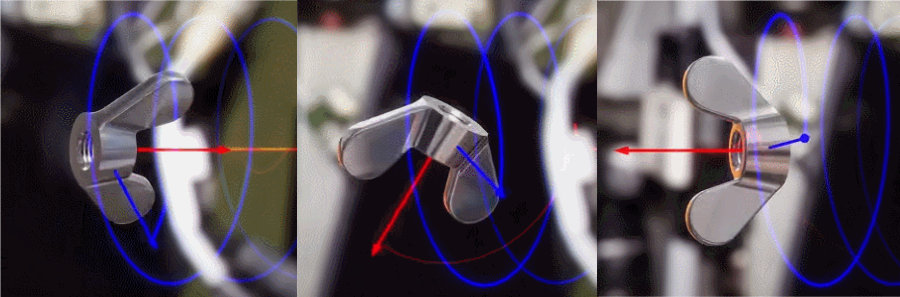
\includegraphics[width=0.9\textwidth]{dzhani.jpg}
\end{center}
   \caption{Изображение эффекта Джанибекова \cite{28}.}
\label{fig:10}
\end{figure*}

Исследование плоскостей сдвига (разломов) в коре Земли (Рисунок \ref{fig:8}), где кора Земли была разрушена или деформирована, также следует тому же шаблону. Феликс Мейнез, голландский геофизик, объясняет в своей статье \cite{36}, что наиболее вероятной причиной этого шаблона является сдвиг оси вращения Земли.

Расположение основных мировых пустынь и центров биоразнообразия также совпадает с этим шаблоном. Пустыни находятся в местах, которые ожидается будут сильно заполнены осадками, в то время как центры биоразнообразия находятся в областях, которые не подвергаются значительным перемещениям океана \cite{28}. Это совпадение показано на Рисунке \ref{fig:9}.

Такие совпадения с предсказанным путем вращения ECDO также существуют в палеотоках осадков, сохранившихся в песчаниковых слоях западных Соединенных Штатов \cite{21}, и в ледниковых валунах, которые были перенесены, вероятно, ледниками, и отложены на основу из породы, отличающейся от самой глыбы. В Великобритании эти валуны следуют ожидаемым путям потоков, соответствующим вращению ECDO \cite{67,68}.

\section{Физика, обуславливающая переворот ECDO}

\begin{figure*}[t]
\begin{center}
\includegraphics[width=1\textwidth]{layers.jpg}
\end{center}
   \caption{Изображение процессов внутри Земли, ведущих к перевороту ECDO \cite{129}.}
\label{fig:11}
\end{figure*}

\begin{figure}[t]
\begin{center}
   \includegraphics[width=1\linewidth]{llvp.jpg}
\end{center}
   \caption{Детально изображено LLVP под Южной Африкой \cite{28}.}
\label{fig:12}
\label{fig:onecol}
\end{figure}

Принцип, лежащий в основе быстрого изменения оси вращения Земли, заключается в физике вращающихся объектов. Каноническим примером этого является эффект Джанибекова, открытый российским космонавтом Владимиром Джанибековым \cite{37}, и изображенный на Рисунке \ref{fig:10}. Объект, который не вращается идеально вокруг одной из своих трёх главных осей инерции, не сохранит фиксированную ось вращения. Если он вращается близко ко второй главной оси, он будет испытывать кажущиеся внезапные сдвиги в вращении. Хотя это не точно то, что, как мы полагаем, происходит во время быстрых переворотов Земли, суть в том, что в отсутствие внешних сил только физика вращения может объяснить быстрое изменение оси вращения Земли.

На самом деле, Земля почти наверняка не испытывает простого и равномерного эффекта Джанибекова. Если бы это было так, мы могли бы обнаружить постепенное изменение оси вращения Земли со временем. Скорее, мы считаем, что Земля испытывает периодические, внезапные нарушения в своей физической структуре, ведущие к разъединению её «внешних вращательных» (кора/мантия) и «внутренних вращательных тел» (ядро). Без внешнего воздействия закон сохранения углового момента утверждает, что Земля не может внезапно изменить свою ось вращения, поэтому разъединение внешних и внутренних вращательных тел является одной из немногих вещей, исключая внешнее воздействие на Землю, которые могут вызвать внезапный и резкий переворот.
Процесс, который вызывает внутренние изменения в Земле, считается изменением состояния структуры железа, составляющего ядро Земли (Рисунок \ref{fig:11}). Внутреннее ядро состоит из гексагонально плотноупакованного железа (Fe) \cite{141}. При переходе этого hcp-Fe в жидкое металлическое состояние, высвобождается кинетическая энергия и происходит его перемещение во внешнее ядро. Эта фазовая перемена снижает магнитную проницаемость ядра, ослабляя геомагнитное поле, и выделяет тепло, создавая структуры LLVP (большие области низкой скорости сдвига) (Рисунок \ref{fig:12}) \cite{38} в мантии и нагревая поверхность Земли через абиссальные океаны. Оба эти явления хорошо документированы в последние столетия и обсуждены далее в этой статье.

Считается, что этот же процесс внутри Земли, происходящий в обратном направлении, также приводит к возвращению к текущему состоянию вращения Земли относительно скоро после переворота.

\section{Доказательства надвигающегося переворота Земли}

Существует веская причина полагать, что мы находимся на грани очередного переворота Земли. Катастрофа не происходила несколько тысячелетий, что соответствует приблизительной частоте этих событий на основе исторических свидетельств и данных. Наиболее убедительные данные, поддерживающие предполагаемый переворот, исходят из последних геомагнитных данных, которые указывают на то, что геомагнитное поле Земли ослабевало приблизительно две тысячи лет. Это ослабление ускоряется и достигает тревожных темпов в последние несколько десятилетий.

На Рисунке \ref{fig:14} изображено геомагнитное поле Земли в 1590 и 2025 годах \cite{125,126}. Как показано на рисунке, поле значительно ослабло.

Другой метрикой для ослабления геомагнитного поля является положение геомагнитного северного полюса (Рисунок \ref{fig:13}). Исторически геомагнитный север располагался в канадской Арктике. Однако за последние несколько столетий он медленно перемещался, и значительно ускорился несколько десятилетий назад. Сейчас он быстро движется в сторону России со скоростью 55 километров в год \cite{124}.

\begin{figure*}[t]
\begin{center}
\includegraphics[width=0.9\textwidth]{saa.jpg}
\end{center}
   \caption{Изображение ослабления геомагнитного поля с 1590 по 2025 год. Рассчитано с использованием моделей gufm1 и IGRF-14 \cite{125,126}.}
\label{fig:14}
\end{figure*}

\begin{figure}[t]
\begin{center}
   \includegraphics[width=1\linewidth]{npw.jpg}
\end{center}
   \caption{Положение геомагнитного северного полюса с 1590 по 2025 год, представлено с шагом в 5 лет \cite{142}.}
\label{fig:13}
\label{fig:onecol}
\end{figure}

\begin{figure}[t]
\begin{center}
   \includegraphics[width=1\linewidth]{ocean-highlight.jpg}
\end{center}
   \caption{Темпы нагрева глубокого ($>$2000 м глубины) океана с 1991 по 2010 год, обведено красным \cite{132}.}
\label{fig:15}
\label{fig:onecol}
\end{figure}

Считается, что магнитное поле Земли генерируется внутренним динамо - круговыми потоками магмы, движущимися в внешнем ядре Земли из-за его вращения \cite{123}. Ослабление геомагнитного поля является симптомом изменений в глубинах Земли. Согласно теории ECDO, эти изменения выбрасывают тепло и в конечном итоге приводят к разделению мантии и ядра, вызывая переворот Земли \cite{1}.
Существует значительное количество данных, подтверждающих наличие экзотермических процессов в недрах Земли. Нагрев Земли документально подтвержден ростом температур поверхности континентов и океанов \cite{127,128}, увеличением уровня CO2 в атмосфере в унисон с тепловыми шлейфами Земли \cite{129,130} и уменьшением площади глобального морского льда \cite{131}. Данные показывают, что рост уровней CO2 и температур не является причиной "антропогенных" изменений климата, а скорее вторичными эффектами экзотермического ядра \cite{129}.

Наиболее значимыми являются исследования темпов нагрева в глубинах океана (глубина $>$2000 метров), которые показывают, что не только глубокие слои океанов нагреваются, но и самые мощные темпы нагрева находятся в абиссальной зоне (4000 - 6000 м). Это глубоководное нагревание имеет центроид ниже 4000 метров \cite{132,129}, что было бы невозможно, если бы океаны нагревались сверху атмосферой. Такие данные предоставляют убедительные доказательства того, что современные климатические и геомагнитные изменения обусловлены процессами, происходящими глубоко внутри Земли. Рисунок \ref{fig:15} изображает глобальные темпы нагрева глубоководных океанов с 1991 по 2010 годы \cite{132}.

\section{Моделирование Предстоящего Переворота Земли}

\begin{figure}[t]
\begin{center}
   \includegraphics[width=1\linewidth]{saa-crop.jpeg}
\end{center}
   \caption{Расчет критической точки на основе Южно-Атлантической аномалии указывает на дату 13 марта 2059 года \cite{125,126}.}
\label{fig:16}
\label{fig:onecol}
\end{figure}

Прогнозирование времени следующего переворота Земли является сложной задачей. В настоящее время лучшая модель для этого заключается в геомагнитном поле Земли - Южно-Атлантической аномалии (SAA). Этот регион над Южной Атлантикой имеет наименьшую геомагнитную силу поля и определяется как область с интенсивностью поля ниже 32,000 нанотесл \cite{135}, что было самым низким значением поля в 1590 году. Площадь поверхности Южно-Атлантической аномалии увеличилась с 1\% площади Земли в 1590 году до 21\% в 2025 году \cite{136}.

Чтобы получить оценку, когда Земля может перевернуться, я сопоставил данные о площади поверхности SAA к уравнению критической точки в виде степенного закона, которое моделирует сложную систему, приближающуюся к критическому переходу, при котором система претерпевает резкое и внезапное изменение. Мои вычисления дали предсказанную дату критической точки 13 марта 2059 года (Рисунок \ref{fig:16}). Это предсказание станет все более и более точным по мере приближения к переходу \cite{136}.

Другие метрики, такие как блуждание оси вращения, погодные аномалии, а также сейсмические и вулканические данные, также могут помочь нам точнее предсказать, когда может произойти следующий переворот Земли.

\section{Историческая Хронология ECDO}

Хотя установление точной хронологии прошедших событий ECDO является сложной задачей, кажется, что во время Голоцена было по крайней мере 2 события ECDO. Обратите внимание на рассказ, переданный Геродотом от египетских жрецов, что, \textit{"от первого царя до этого последнего священника Гефеста прошло триста сорок одно поколение людей... В это время они сказали, что солнце четыре раза перемещалось из своего привычного места восхода, и где оно сейчас заходит, там дважды было его восходом, и там, откуда оно сейчас восходит, было дважды его заходом"} \cite{32}. Платон, живший в пятом веке до нашей эры \cite{111}, заявил, что после потопа, который затопил Атлантиду за один день и ночь за 9,000 лет до этого, \textit{"после этого произошло много потопов, и остатки, выжившие в горах, не знали искусства письма, и в течение многих поколений были полностью преданы приобретению средств к жизни"} \cite{112}, что предполагает, что было больше двух переворотов с конца Младшего Дриаса около 9700 года до нашей эры. Физические доказательства, описанные по ходу всей этой работы и в моих исследованиях \cite{2}, предоставляют достаточные свидетельства рассказа Платона.

Наиболее вероятная дата смены ЭКДО приходится на период с 2300 по 1600 годы до н.э., к которому относятся многие катастрофические наводнения (Гун-Юй \cite{113,114,115}, Огиг \cite{116,117}, Перу \cite{118,119}, Исход \cite{120}), разрушения и заброшенности цивилизаций (Мохенджо-Даро \cite{121}, минойский Крит \cite{100,101}) и физические аномалии (события бонд \cite{122}, событие 4,2 тысячи лет \cite{90}). Нет достаточного совпадения доказательств, более поздних, чем этот период, указывающих на крупное катастрофическое событие.

\section{Заключение}

Операция NANOOK была разведывательной операцией времен холодной войны США по картированию Арктики и северного побережья Советского Союза после Второй мировой войны \cite{137}. В ходе их исследования было обнаружено, что магнитный полюс находился на 125–200 миль севернее, чем предполагалось на основе данных предыдущих экспедиций. Соответственно, \textit{"Среди правительственных ученых возник вопрос о том, что будет, когда магнитные и географические полюсы совпадут. Чтобы ответить на это, под руководством доктора Пола А. Сайпла корпорации Rand был заключен контракт на проведение лабораторных исследований, в ходе которых были построены модели Земли из концентрических сфер: внутренняя сфера представляла собой электромагнитно заряженное расплавленное железное ядро Земли, ось которого определяла “магнитные” полюсы; и внешняя сфера представляла собой кору Земли, которая вращалась вокруг “географической” полярной оси. Было выявлено в результате повторных экспериментов, что по мере приближения “магнитного” полюса к “географическому” полюсу в какой-то момент “магнитный” полюс ускорит скорость своего сближения, как будто его притягивает к “географическому” полюсу центростремительная сила и прыгнет для совпадения; но вместо совпадения полюсов “магнитный” полюс быстро “перевернется” вокруг “географического” полюса, а затем стремительно переместится к экватору, как бы под воздействием центробежной силы, оказавшись в положении, где обе оси приняли приблизительное 89-градусное расхождение. После этого произошедшего полярного “перевертывания” оси затем постепенно начнут вновь сходиться в течение длительного времени"} \cite{138,139}.

Впоследствии, \textit{"На одном из научных совещаний, которые майор Уайт посетил в Пентагоне в начале 1948 года, ученые обсуждали целесообразность информирования общественности о надвигающемся явлении полярного переворота. Ни один из ученых не согласился скрыть информацию от общественности; но, с другой стороны, они не смогли прийти к соглашению о том, как ее раскрыть. Знание об этом феномене, как считают некоторые, само по себе могло бы разрушить моральные устои общества. Их страхи, по-видимому, не оправдались, когда в начале 1950-х годов информация о феномене переворота была опубликована как в газетной колонке, так и в журнальной статье, но неожиданно не вызвала никакого отклика от явно ошеломленной, локальной или недоверчивой общественности"} \cite{138,139}.

Почему мы не обращаем на это внимание? Есть много причин полагать, что Земля переворачивалась раньше. Эта статья вместе с частью второй работы предоставляет насыщенное резюме большого совпадения доказательств из множества областей, указывающих на то, что это так, например, рассказы о наводнениях по всему миру, солевые и морские окаменелости, покрывающие континенты, древние подземные убежища, останки животных и катастрофические геологические ландшафты. Человечество, как предполагается, существует сотни тысяч лет, но современная история охватывает лишь несколько тысячелетий. Разве не может так быть, что время от времени Земля переворачивается, континенты очищаются, и мы вынуждены вернуться к точке отсчета – каменному веку, сведя наши записи древней истории до горстки катастрофических повествований? Если это так, то предотвращение повторного возникновения этого может стать одной из важнейших задач человечества.

В заключение, я оставлю вас с этой историей, рассказанной в "Тимее", написанном Платоном, о разговоре между Солоном, афинским государственным деятелем, и египетскими жрецами \cite{140}: \textit{"И однажды, когда [Солон] желал, чтобы они говорили о древней истории, он попытался рассказать им наши наиболее древние предания, касающиеся Форонея, которого называли первым человеком, и Ниобу; и он продолжал рассказывать легенду о Девкалионе и Пирре после Потопа, и как они его пережили, и дать генеалогию их потомков; и, подсчитывая количество лет, занятых упомянутыми событиями, пытался вычислить периоды времени. Где один из жрецов, чрезвычайно старый человек, сказал: "О Солон, Солон, вы, греки, всегда дети: нет такого явления как старый грек." И, услышав это, он спросил: "Что ты имеешь в виду под этими словами?" И жрец ответил: "Вы молоды душой, все до одного. Ибо в этом у вас нет ни одной веры, которая была бы древней и унаследованной от древней традиции, ни одной науки, которая была бы седовласой от возраста. И это причина того: было и будет много и различных разрушений человечества, из которых большие происходят от огня и воды, а меньшие — от бесчисленных других способов. Ведь на самом деле история, которая рассказывается в вашей стране, как и в нашей, как Фаэтон, сын Гелиоса, однажды запряг колесницу своего отца и, поскольку он не мог вести её по пути, по которому шёл его отец, сжёг всё, что было на земле, и сам погиб от удара молнии — эта история, как её рассказывают, имеет вид легенды, но истина её заключается в смещении тел на небесах, которые вращаются вокруг земли, и разрушении вещей на земле от неистового огня, который повторяется через длительные интервалы. В такие времена все, кто живет в горах и на возвышенных и сухих местах, терпят разрушения больше, чем те, кто живет рядом с реками или морем; и в нашем случае Нил, наш Спаситель другими способами, спасает нас также в такие времена от этого бедствия, поднимаясь высоко. А когда, с другой стороны, Боги очищают землю потопом вод, все скотоводы и пастухи, находящиеся в горах, спасаются, но те, кто в городах вашей страны, уносятся потоками в море; тогда как в нашей стране ни тогда, ни в любое другое время вода не льется на наши поля сверху, напротив, она вся склонна естественным образом исходить из-под земли. Отсюда по этим причинам то, что здесь сохраняется, считается наиболее древним; истина заключается в том, что в каждом месте, где нет чрезмерной жары или холода, всегда существуют какие-то человеческие роды, то больше, то меньше в числе. И если произошло какое-то событие, благородное или великое, или любым образом заметное, будь то в вашей стране, или в нашей, или в каком-то другом месте, о котором мы знаем по слухам, все такие события записываются с давних пор и сохраняются здесь, в наших храмах; тогда как ваши люди и другие каждый раз ново обустраиваются буквами и всеми такими искусствами, которые требуют цивилизованные государства, и когда, после обычного интервала лет, словно чума, на ваш народ снова обрушивается потоп с небес, он не оставляет никого, кроме неграмотных и нецивилизованных, так что вы становитесь юными, как всегда, без знания всего, что произошло в стародавние времена в этой стране или в вашей. Безусловно, родословные, которые ты только что привел, Солон, касающиеся людей твоей страны, мало чем лучше детских сказок; во-первых, вы помните только один потоп, хотя до этого было много других; и, во-вторых, вы не осведомлены о том, что самое благородное и совершенное человеческое племя родилось на земле, где вы теперь живете, и от них родились и вы сами, и все ваше существующее городское образование, из какого-то маленького семени, которое случайно осталось; но это ускользнуло от вашего внимания, потому что на протяжении многих поколений выжившие умирали, не имея возможности выражать себя письменно. Поистине, однажды, Солон, до самого великого разрушения водой, то, что теперь является Афинским государством, было самым смелым в войне и также превосходно организованным во всех иных отношениях. Говорят, что оно обладало самыми великолепными произведениями искусства и самой благородной политией из всех наций под небесами, о которых мы слышали”}.

Эти же священники, конечно, рассказывали Солону об античной цивилизации Атлантиды: \textit{"Ибо все, что у нас здесь, лежащее в устье, о котором мы говорим, очевидно, является гаванью с узким входом; но там дальше – это настоящий океан, и землю, окружающую его, можно справедливо назвать в полном и истинном смысле континентом. Теперь на этом острове Атлантида существовала конфедерация царей великой и удивительной власти, которая господствовала над всем островом, а также над многими другими островами и частями континента; и, кроме того, на землях внутри пролива они правили Ливией до Египта и Европой до Тиррении. Итак, это войско, собравшись вместе, однажды попыталось подчинить одним единственным ударом обе ваши страны и наши, и всю территорию внутри пролива. Именно тогда, Солон, мужество вашего государства проявилось выдающейся доблестью и силой на глазах у всего мира. Оно выделялось выше всех в храбрости и во всех военных искусствах, и, действуя частично как лидер греков, а частично стоя в одиночестве, когда было оставлено всеми другими, пройдя самые смертельные опасности, оно разбило захватчиков и установило трофей; благодаря чему оно спасло от рабства тех, кто еще не был порабощен, а всех остальных из нас, кто обитает в пределах Геркулесовых столбов, оно щедро освободило. Но позднее произошли чудовищные землетрясения и наводнения, и один тяжкий день и ночь постигли их, когда все воины вашего народа были поглощены землей, а остров Атлантида подобным образом был поглощен морем и исчез"}.

\section{Благодарности}

Благодарности направлены Эрическому Скетпику, первоначальному автору теории ECDO, за завершение его проницательной, новаторской диссертации и её распространение по миру. Его тройная диссертация \cite{1} по-прежнему остается основополагающей работой в теории расслоения экзотермического ядра и мантии (ECDO), и содержит гораздо больше информации по теме, чем я кратко осветил здесь.

Благодарности Анкиту, который обработал данные компиляции катаклизмов в Таблице 1.

И, конечно, благодарности гигантам, на чьих плечах мы стоим; тем, кто провел все исследования и расследования, которые сделали эту работу возможной, и трудился, чтобы принести свет человечеству.

\clearpage
\twocolumn

\section{Дополнительные изображения}

\begin{figure}[H]
\begin{center}
   \includegraphics[width=1\linewidth]{wave.jpg}
\end{center}
   \caption{Ближний взгляд на подрезку, параболическую эрозию волн на пирамиде Хафры \cite{27}.}
\label{fig:19}
\label{fig:onecol}
\end{figure}

\begin{figure}[H]
\begin{center}
   \includegraphics[width=1\linewidth]{star-stone.jpg}
\end{center}
   \caption{Карта звезд, вырезанная на камне в одном из шахт пирамиды Хуфу \cite{28}.}
\label{fig:20}
\label{fig:onecol}
\end{figure}

\begin{figure*}[t]
\begin{center}
\includegraphics[width=1\textwidth]{deepsea.jpg}
\end{center}
   \caption{Визуализация аномалии нагрева глубокого и абиссального океана по сравнению с нормальной кривой нагрева атмосферного океана. Общая аномалия нагрева взята из NOAA \cite{147}, распределение нагрева в глубине и абиссах из исследования Дебрюера \cite{132}, а обработка данных и визуализация выполнены Этическим СкеПтиком \cite{129}.}
\label{fig:21}
\end{figure*}

\begin{figure*}[t]
\begin{center}
\includegraphics[width=1\textwidth]{sealevel.jpeg}
\end{center}
   \caption{Уровень моря показывает 20\% увеличение дисперсии за 75 лет по 63 станциям, указывая на повышение скорости течения. Взмывания дисперсии уровня моря совпадают с тепловыми импульсами океана, указывая на то, что это может быть вызвано нагреванием из глубины океанов Земли \cite{2,129}.}
\label{fig:22}
\end{figure*}
\begin{figure*}[t]
\begin{center}
\includegraphics[width=1\textwidth]{co2.jpg}
\end{center}
   \caption{Количество CO2 в атмосфере (ppm) неуклонно росло за последние 45 лет, вероятно, из-за повышения температуры океана. Источник: NOAA \cite{148,129}.}
\label{fig:23}
\end{figure*}

\begin{figure*}[t]
\begin{center}
\includegraphics[width=1\textwidth]{ice.jpg}
\end{center}
   \caption{Общая площадь морского льда сокращалась за последние 45 лет из-за потепления Земли. Источник: ADS \cite{149}.}
\label{fig:24}
\end{figure*}

\clearpage
\twocolumn

{\small
\bibliographystyle{ieee}
\bibliography{egbib}
}

\end{document}
